\documentclass{svmult}

\usepackage{mathptmx}       % selects Times Roman as basic font
\usepackage{helvet}         % selects Helvetica as sans-serif font
\usepackage{courier}        % selects Courier as typewriter font
\usepackage{type1cm}        % activate if the above 3 fonts are
                            % not available on your system
\usepackage[numbers]{natbib}
%
\usepackage{makeidx}         % allows index generation
\usepackage{graphicx}        % standard LaTeX graphics tool
                             % when including figure files
\usepackage{multicol}        % used for the two-column index
\usepackage[bottom]{footmisc}% places footnotes at page bottom
\usepackage{listings}
\usepackage{color}
\usepackage{tikz}
\usepackage{amsmath}
\usepackage{amssymb}

\usepackage{footmisc}
\usepackage{import}
\usepackage{enumitem}
\usepackage{booktabs}
\usepackage{lipsum}

\usepackage{capt-of}
\usepackage{float}
\usepackage{tabularx}
\usepackage{watermark} % titlepage image
\usepackage{booktabs}
\usepackage[hidelinks]{hyperref}
\usepackage[parfill]{parskip}
%\usepackage[nottoc]{tocbibind}
\usepackage{tocloft}
\usepackage[disable]{todonotes}

\usepackage{microtype} % Improves spacing
\usepackage{fancyhdr} 
\fancyhead[L]{\rightmark}
\fancyhead[R]{\leftmark} 
\usepackage[toc,page]{appendix}

\usetikzlibrary{shapes.misc, shapes.geometric, arrows, positioning, calc, decorations.markings}
\tikzset{
  query/.style={draw=blue!10,thick,fill=blue!2,inner sep=.15cm},
  answer/.style={rectangle,draw=black!10,fill=gray!4},
  icon/.style={circle,thick,fill=blue!20,draw=blue!30,inner sep=.05cm,font=\bfseries},
  data/.style={draw=easeblue!30,thick,fill=easeblue!10,inner sep=.15cm},
  owlclass/.style={draw=easeblue!40,fill=easeblue!10,text=easeblue,font=\bf,minimum width=2.5cm},
  owlclass_f/.style={owlclass,text width=2.0cm,minimum width=2.0cm,text badly centered},
  relation/.style={thick,-latex,black,font=\it\scriptsize},
  relationxl/.style={relation,bend right=20},
  relationxr/.style={relation,bend left=-20},
}
\pgfdeclarelayer{back}
\pgfdeclarelayer{front}
\pgfsetlayers{back,main,front}

\lstdefinelanguage[OWL]{XML} {morekeywords={Individual,ObjectProperty,Types,Facts,Class,SubClassOf,Domain,Range,SubPropertyOf,EquivalentTo}}
\lstdefinestyle{OWL}    {language=[OWL]XML,    lineskip=0.2ex, fontadjust=true, basicstyle={\scriptsize \nopagebreak[4]}}
\lstdefinestyle{Prolog} {language=Prolog, lineskip=0.2ex, fontadjust=true, basicstyle={\scriptsize \nopagebreak[4]}, commentstyle=\scriptsize,
    morekeywords={entity, occurs, holds, show, append, forall, findall, member}}

\graphicspath{img}

\lstdefinestyle{lispcode}{
	backgroundcolor=\color{lightgray},   
	commentstyle=\color{codegreen},
	keywordstyle=\color{magenta},
	numberstyle=\tiny\color{white},
	stringstyle=\color{purple},
	basicstyle=\ttfamily\footnotesize,
	breakatwhitespace=false,         
	breaklines=true,                 
	captionpos=b,                    
	keepspaces=true,                 
	numbers=left,                    
	numbersep=5pt,                  
	showspaces=false,                
	showstringspaces=false,
	showtabs=false,                  
	tabsize=2
}

\definecolor{ease_lightblue}{HTML}{D4E5EF}
\definecolor{ease_darkblue}{HTML}{144F78}
\colorlet{easeblue}{ease_darkblue}
\colorlet{robotblue}{ease_darkblue}

% json data display 
\colorlet{json_punctuation}{red!60!black}
\definecolor{json_background}{HTML}{EEEEEE}
\definecolor{json_delim}{RGB}{20,105,176}
\colorlet{json_numb}{magenta!60!black}

\lstdefinelanguage{json}{
	basicstyle=\normalfont\ttfamily,
	numbers=left,
	numberstyle=\scriptsize,
	stepnumber=1,
	numbersep=8pt,
	showstringspaces=false,
	breaklines=true,
	frame=lines,
	backgroundcolor=\color{json_background},
	literate=
	*{0}{{{\color{json_numb}0}}}{1}
	{1}{{{\color{json_numb}1}}}{1}
	{2}{{{\color{json_numb}2}}}{1}
	{3}{{{\color{json_numb}3}}}{1}
	{4}{{{\color{json_numb}4}}}{1}
	{5}{{{\color{json_numb}5}}}{1}
	{6}{{{\color{json_numb}6}}}{1}
	{7}{{{\color{json_numb}7}}}{1}
	{8}{{{\color{json_numb}8}}}{1}
	{9}{{{\color{json_numb}9}}}{1}
	{:}{{{\color{json_punctuation}{:}}}}{1}
	{,}{{{\color{json_punctuation}{,}}}}{1}
	{\{}{{{\color{json_delim}{\{}}}}{1}
	{\}}{{{\color{json_delim}{\}}}}}{1}
	{[}{{{\color{json_delim}{[}}}}{1}
	{]}{{{\color{json_delim}{]}}}}{1},
}

%\newcommand{\todo}[1]{\textcolor{red}{\textbf{TODO}: #1}}
%\lstdefinelanguage[OWL]{XML} {morekeywords={Individual,ObjectProperty,Types,Facts,Class,SubClassOf,Domain,Range,SubPropertyOf,EquivalentTo}}
%\lstdefinestyle{OWL}    {language=[OWL]XML,    lineskip=0.2ex, fontadjust=true, basicstyle={\scriptsize \nopagebreak[4]}}
%\lstdefinestyle{Prolog} {language=Prolog, lineskip=0.2ex, fontadjust=true, basicstyle={\scriptsize \nopagebreak[4]}, commentstyle=\scriptsize,
%    morekeywords={entity, occurs, holds, show, append, forall, findall, member}}

\title*{NEEM Generation Checklist}
\author{
   Daniel Be{\ss}ler,
   Sebastian Koralewski,
   Abhijit Vyas,
   Kaviya Dhanabalachandran,
   Sascha Jongebloed
}
\authorrunning{Beetz et al.}
\institute{CRC Everyday Activity Science and Engineering (EASE)\\ University Bremen, Am Fallturm 1, 28359 Bremen\\ \texttt{ai-office@cs.uni-bremen.de}}
\thiswatermark{
 \centering
 \put(0,-630){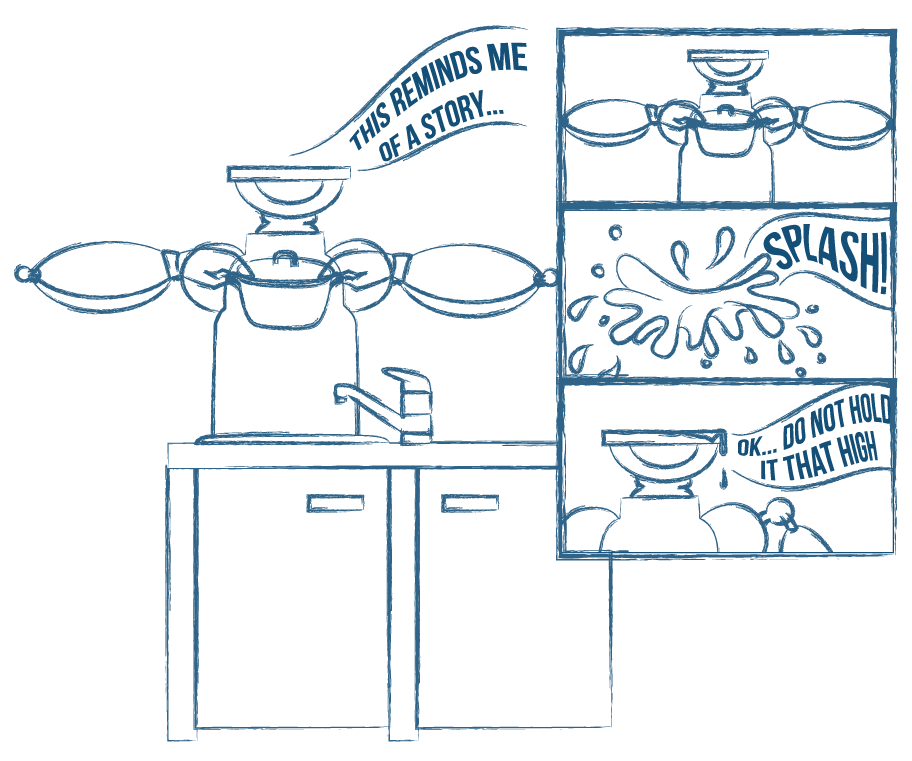
\includegraphics[width=12cm]{img/NarrativesStory.png}}
 \put(340,-10){
\includegraphics[width=4.0cm]{img/ease-logo.pdf}}}

\renewcommand\thesection{\thechapter.\arabic{section}}

% TODO: use current SOMA version?
\newcommand{\neemversion}{1.0~}
\newcommand{\neemexp}{NEEM-experience~}
\newcommand{\neemexps}{NEEM-experiences~}
\newcommand{\neemnar}{NEEM-narrative~}
\newcommand{\neembak}{NEEM-background~}
\newcommand{\neem}{NEEM~}
\newcommand{\neems}{NEEMs~}
\newcommand{\neemhub}{NEEM-hub~}
\newcommand{\tf}{tf~}
\newcommand{\openease}{openEASE~}
\newcommand{\ease}{EASE~}
\newcommand{\mongodb}{MongoDB~}
\newcommand{\cram}{CRAM~}
\newcommand{\knowrob}{KnowRob~}
\newcommand{\owl}{OWL~}
\newcommand{\pr}{PR2~}
\newcommand{\qudt}{Qudt~}
\newcommand{\boxy}{Boxy~}
\newcommand{\eg}{e.g.~}
\newcommand{\ros}{ROS~}
\newcommand{\soma}{SOMA~}
\newcommand{\dul}{DUL~}
\newcommand{\easeOwl}{EASE.owl~}
\newcommand{\easeAct}{EASE-ACT.owl~}
\newcommand{\easeObj}{EASE-OBJ.owl~}
\newcommand{\cramOwl}{cram\_failures.owl}
\newcommand{\cramentitytoreplace}[1]{\textless #1\textgreater}
\newcommand{\cramloggerpackage}{"cram-cloud-logger"~}
\newcommand{\owlClass}[1]{\textit{#1}}
\newcommand{\owlPredicate}[1]{\textit{#1}}
\newcommand{\f}{\mkern-2mu f\mkern-3mu}
\newcommand{\abox}{\mathcal{A}}
\newcommand{\tbox}{\mathcal{T}}
\newcommand{\concept}[1]{\emph{#1}}
\newcommand{\relation}[1]{\emph{#1}}

\makeatletter
\newcommand{\chapterauthor}[1]{%
  {\parindent0pt\vspace*{-25pt}%
  \linespread{1.1}\large\scshape#1%
  \par\nobreak\vspace*{35pt}}
  \@afterheading%
}
\makeatother

\renewcommand\tabularxcolumn[1]{m{#1}}
\newcolumntype{Y}{>{\centering\arraybackslash}X}
% % % % % % % % % % % % % % % % % % % % % % % %
% % % Prelude
% % % % % % % % % % % % % % % % % % % % % % % %
\newcommand{\givenODPNAME}{}
\newcommand{\givenODPINTENT}{}
\newcommand{\givenODPDEFINEDIN}{}
\newcommand{\givenODPGRAPHIC}{}
\newcommand{\givenODPEXAMPLES}{}
\newcommand{\givenODPQUESTION}{}
\newcommand{\ODPINTENT}[1]     {\renewcommand{\givenODPINTENT}{#1}}
\newcommand{\ODPDEFINEDIN}[1]  {\renewcommand{\givenODPDEFINEDIN}{#1}}
\newcommand{\ODPGRAPHIC}[1]    {\renewcommand{\givenODPGRAPHIC}{#1}}
\newcommand{\ODPEXAMPLES}[1]   {\renewcommand{\givenODPEXAMPLES}{#1}}
\newcommand{\ODPQUESTION}[1]   {\renewcommand{\givenODPQUESTION}{#1}}
\newcommand{\OPDinit}{
  \renewcommand{\givenODPINTENT}{REQUIRED!}
  \renewcommand{\givenODPDEFINEDIN}{REQUIRED!}
  \renewcommand{\givenODPGRAPHIC}{REQUIRED!}
  \renewcommand{\givenODPQUESTION}{}
  \renewcommand{\givenODPEXAMPLES}{}
  \renewcommand{\labelitemi}{$\mathbf{\sqsubseteq}$}
}

\newenvironment{ODP}[1]{
\OPDinit
\renewcommand{\givenODPNAME}{#1}
}{
%\givenODPDESCRIPTION
%\begin{figure}[htb!]
\vspace{0.2cm}
\begin{minipage}{0.55\textwidth}
\fcolorbox{easeblue!40}{easeblue!10}{\begin{tabular}{ p{1.8cm} p{4.2cm} }
%\toprule
% {\it\bf Name}                 & \emph{\givenODPNAME} \\
{\noindent\color{easeblue}\it\bf Intent}               & \givenODPINTENT \\
{\noindent\color{easeblue}\it\bf Competency Questions} & \emph{\givenODPQUESTION} \\
{\noindent\color{easeblue}\it\bf Defined in}           & \givenODPDEFINEDIN \\
%\bottomrule
\end{tabular}}
\end{minipage}
\begin{minipage}{0.45\textwidth}
\begin{center}
\givenODPGRAPHIC
\end{center}
\end{minipage}
\\[0.4cm]
\fcolorbox{easeblue!40}{easeblue!10}{
	\begin{minipage}{0.96\textwidth}
		\begin{tabular}{p{4.4cm}p{6.7cm}}
		{\noindent\color{easeblue}\it\bf Expression}  &
		{\noindent\color{easeblue}\it\bf Meaning} \\
		\givenODPEXAMPLES
		\end{tabular}
	\end{minipage}
}
%\caption{\emph{The Representation of \givenODPNAME}.}
%\end{figure}
\vspace{0.2cm}
}

\setcounter{tocdepth}{3}

\begin{document}
\let\oldaddcontentsline\addcontentsline
\def\addcontentsline#1#2#3{}
\maketitle 

\begin{abstract}
This document will present the \neem generation checklist which should be referred by creator of new \neem. 
\end{abstract}

\setcounter{section}{0}
\chapter{NEEM Quick-start Guide}
\label{ch:initial_checklist}

In this chapter we give a checklist for the \neems creation process to help the users in generating \neems in case no existing NEEM-logger can be used. 

\section{NEEM Checklist}

\subsection{Necessary files}
\label{sec:checklist_files}

You should have the following files available:

\begin{itemize}
	\item Agent meshes and urdf files are available
	\item Agent owl file corresponding to urdf needs to be created
	\begin{itemize}
		\item Required kinematic information is provided in owl file pointing to correct urdf file name 
	\end{itemize}
	\item Environment meshes and urdf files are available
	\item Environment owl file corresponding to urdf needs to be created
	\begin{itemize}
		\item Required kinematic information is provided in owl file pointing to correct urdf file name
	\end{itemize}
\end{itemize}

\subsection{Data formats}

The data should automatically be in the correct format if KnowRob is used to log the tf and triple information. If the data was recorded without using Knowrob, please follow the checklist below:

\begin{itemize}
	\item Make sure if tf data is available in correct format
	\begin{itemize}
		\item Tf data is provided as individual json documents not as the list/array of json documents.
		\item The coordinate system is right handed
		\item Correct tf tree is presented in the data
		\item Joint rotation is provided in quaternion
		\item Position data is logged in meters
	\end{itemize}
	\item Make sure if triple data is available in correct format
	\begin{itemize}
		\item Triple data is provided as an array of json document
		\item Correct \soma concepts used from \neemnar part
	\end{itemize}
\end{itemize}

\subsection{Semantic Annotation}
\label{sec:semantic_annotation}

In this chapter we discuss the necessary semantic annotation that is stored in the triple collection. First we will list the semantic information that is necessary to generate a simple NEEM:

\begin{itemize}
	\item Necessary steps when starting the logging:
	\begin{itemize}
		\item Create the episode and add dul:isSettingFor relation between the episode and the robots and locations (see \ref{sec:episodes})
	\end{itemize}
	\item Create an hierachy of actions
	\begin{itemize}
		\item Add the task that is executed during the action (see \ref{sec:classification})
		\item Add start and endtime (as unix timestamps) to action (see \ref{sec:occurrences})
		\item Repeat the above points for all sub-actions of the Action-Hierachy, and link them to the parent-actions (see \ref{sec:composition})
		\item For the top-level action: Link the action to the created Episode
	\end{itemize}
\end{itemize}

Now we we will list some additional semantic annotation that would be helpful for the future use of the logged NEEM:

\begin{itemize}
	\item Add additional informations to better classify an action: 
	\begin{itemize}
		\item Add the performing agents (see \ref{sec:participation})
		\item Add objects that are participating in the action (see \ref{sec:participation})
		\item Add conceptualization to the objects in an action by adding roles (see \ref{sec:narrative:roles})
		\item Add executed motions to an action (see \ref{sec:narrative:events})
	\end{itemize}
\end{itemize}

In general, additional semantic annotations can be added as needed. In the next chapter we show how this annotation can be implemented with KnowRob.

\subsection{Semantic Annotation: KnowRob}
\label{sec:semantic_annotation_knowrob}

The easiest way to generate a correct semantic annotation described in \ref{sec:semantic_annotation} is using KnowRob. First we will describe which queries are necessary to generate a simple NEEM. The used concepts for agents, objects, roles etc. are examples. Please find the correct concepts for your usage in SOMA\footnote{https://ease-crc.github.io/soma}.

\begin{itemize}
	\item Necessary steps when starting the logging:
	\begin{itemize}
		\item Load the OWL Files collected according to \ref{sec:checklist_files}, e.g.: 
			\begin{lstlisting}[language=Prolog]
tripledb_load('package://knowrob/owl/robots/PR2.owl')
			\end{lstlisting}
		\item Load the URDF Files and link them to the corresponding robot/location from the OWL File, e.g.:
		\begin{lstlisting}[language=Prolog]
urdf_load('http://knowrob.org/kb/PR2.owl#PR2_0', 'package://knowrob/urdf/pr2.urdf', [load_rdf])
		\end{lstlisting}
		\item Create the episode: tell(is\_episode(Episode))
		\item Add setting\_for relations for robots and locations: 
		\begin{lstlisting}[language=Prolog]
is_setting_for(Episode,'http://knowrob.org/kb/PR2.owl#PR2_0')
		\end{lstlisting}
	\end{itemize}
	\item Log the Action-Hierachy
	\begin{itemize}
		\item Create an action, e.g.:
			\begin{lstlisting}[language=Prolog]
tell(is_action(Action))
			\end{lstlisting}
		\item Add the task that is executed during the action, e.g.: 
			\begin{lstlisting}[language=Prolog]
tell([has_type(Tsk,soma:'Transporting'),
executes_task(Action,Tsk)])
			\end{lstlisting}
		\item Add start and endtime (as unix timestamps) to action, e.g.: 
			\begin{lstlisting}[language=Prolog]
tell(occur(Act) during [Start, End])
			\end{lstlisting}
		\item Repeat the above points for all sub-actions of the Action-Hierachy, and link them to the parent-actions:
			\begin{lstlisting}[language=Prolog]
tell(has_subevent(ParentAct,Action))
			\end{lstlisting}
		\item For the top-level action: Link the action to the created Episode, e.g.: 
			\begin{lstlisting}[language=Prolog]
tell(is_setting_for(Episode,Action))
			\end{lstlisting}
	\end{itemize}
\end{itemize}

Now we we will list some additional semantic annotation to add more information to the logged NEEM:

\begin{itemize}
	\item Add additional informations to better classify an action: 
	\begin{itemize}
		\item Add the performing agents, e.g.:
			\begin{lstlisting}[language=Prolog]
tell(is_performed_by(Action,pr2:'PR2_0'))
			\end{lstlisting}
		\item Add objects that are participating in the action, e.g.:
			\begin{lstlisting}[language=Prolog]
tell(has_participant(Action,soma:'Milk_0'), \)
			\end{lstlisting}
		\item Conceptualize objects and agents in an action by adding roles, e.g.:
			\begin{lstlisting}[language=Prolog]
tell([has_type(RobotRole, soma:'AgentRole'),' 
		has_role(pr2:'PR2_0', RobotRole) during Action,'])
			\end{lstlisting}
		\item Add executed motions to an action, e.g.:
			\begin{lstlisting}[language=Prolog]
tell([has_type(Mot,soma:'LimbMotion'),
       is_classified_by(Action,Mot)])
			\end{lstlisting}
	\end{itemize}
\end{itemize}

%\subsection{Checks}
%
%\todo{Should this points stay, or do we hope for automatic neem validation in the neemhub?}
%
%You can try the following checks to test if your logged data is correct:
%
%\begin{itemize}
%	\item Validate triple data with \neem validation script??
%	\item Test current neem experiment data (tf, triple, meshes and urdfs) locally with \knowrob, \todo{here not everyone will use knowrob, so some way we need to provide an interface}
% 	\item Agent and environment meshes with urdf files are rendered properly with \knowrob in rviz 
%\end{itemize}



\cleardoublepage
\setcounter{section}{0}
\chapter{NEEM Data}
\label{ch:acquisition}
\chapterauthor{A. Vyas, S. Jongebloed}

This chapter focuses on the data format expected for process of \neems creation.
At first, we will provide the basic overview how \neem should look like and then will describe ways to create \neems compatible with current \openease and \knowrob.
 

\section{NEEM Structure}
\todo{Talk about the directory structure how how neem should look like and what individual directories means, e.g. tf, triple, annotation & inferred}

\todo{Describe tf and triple data format}


\section{NEEM Creation Process}

\todo{Describe how neems can be created either directly using Knowrob or providing json files for tf and triple data via REST interface(@Sascha, we need to think about this first, how the REST interface should look like?)}



\pagenumbering{arabic}
\setcounter{page}{0}
\cleardoublepage

\end{document}
